
\begin{frame}{Making smart contract smarter~\cite{luu2016making}}

\begin{itemize}
\item Describe security bugs in smart contract development:
\begin{itemize}
\item Transaction-ordering dependence (TOD)
\item Timestamp dependence
\item Mishandled exception
\item Reentrancy vulnerability
\item A survey on vulnerabilities and attacks~\cite{bib:atzei}
\end{itemize}
\item Recommendations for Better Semantics
\begin{itemize}
\item Guarded Transactions: add premise $\sigma \vdash g$
\item Prefer \texttt{block.number} to \texttt{block.timestamp}
\item Better Exception Handling
\end{itemize}


\item Formalized operational semantics:
\begin{itemize}
\item Formation and Validation of blocks
\item Transaction Execution
\item EtherLite: formalization of the EVM instructions
\end{itemize}
\end{itemize}

\end{frame}

\begin{frame}{Making smart contract smarter~\cite{luu2016making}}
\begin{itemize}
\item Architecture of \textbf{OYENTE}:
%\item Since the proposed update require that \emph{all} clients update
\end{itemize}
\begin{center}
	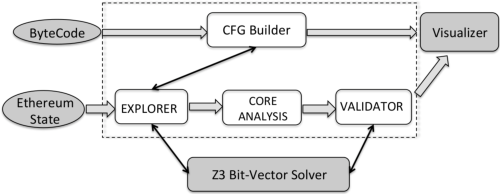
\includegraphics[width=\textwidth]{./img/oyente-architecture.pdf}
\end{center}
\end{frame}

\begin{frame}{Oyente Drawbacks}
They are described in~\cite{grishchenko2018semantic,bib:securify}
\begin{itemize}
\item Luu et al., considers only a variation of a subset of EVM bytecode: e.g. do not consider CREATE instruction
\item Some checks are neither sound nor complete (e.g. ISZERO check)
\item Conceptual flow: 
\begin{itemize}
\item global state non-included in the activation records of the call stack
\end{itemize}
\item False positives and false negatives
\end{itemize}

\end{frame}